

\begin{multicols}{2}
\textbf{Ingredients}
\begin{itemize}
\item 2 red bell peppers

\item 1 lb green beans  
\item 2 chicken breasts
\item 1 can coconut milk
\item 1 can thai red curry paste 
\item lime juice
\item ginger paste
\item minced garlic (~6 cloves) 
\item basil 
\item salt to taste



\end{itemize}


\columnbreak
\textbf{Procedure:}
\medskip


\begin{enumerate}

\item Cut the bell peppers into strips and remove the stems from the green beans. Cube the chicken breast and sautee in a pan until cooked through. Remove from heat. 
\medskip

\item While the chicken is cooking, add the garlic, ginger, and red curry paste to a pan with some olive oil on a medium heat and cook until fragrant. Add the can of coconut milk, red bell peppers, and green beans and bring to medium-high temp, stirring occasionally. 
\newline 

 \item Cook the vegetables until they are soft and then add the chicken back to the mix. Cook for another few minutes and add salt,  lime juice, and basil to taste. Serve over jasmine rice. 
\end{enumerate}
\end{multicols}
\centering 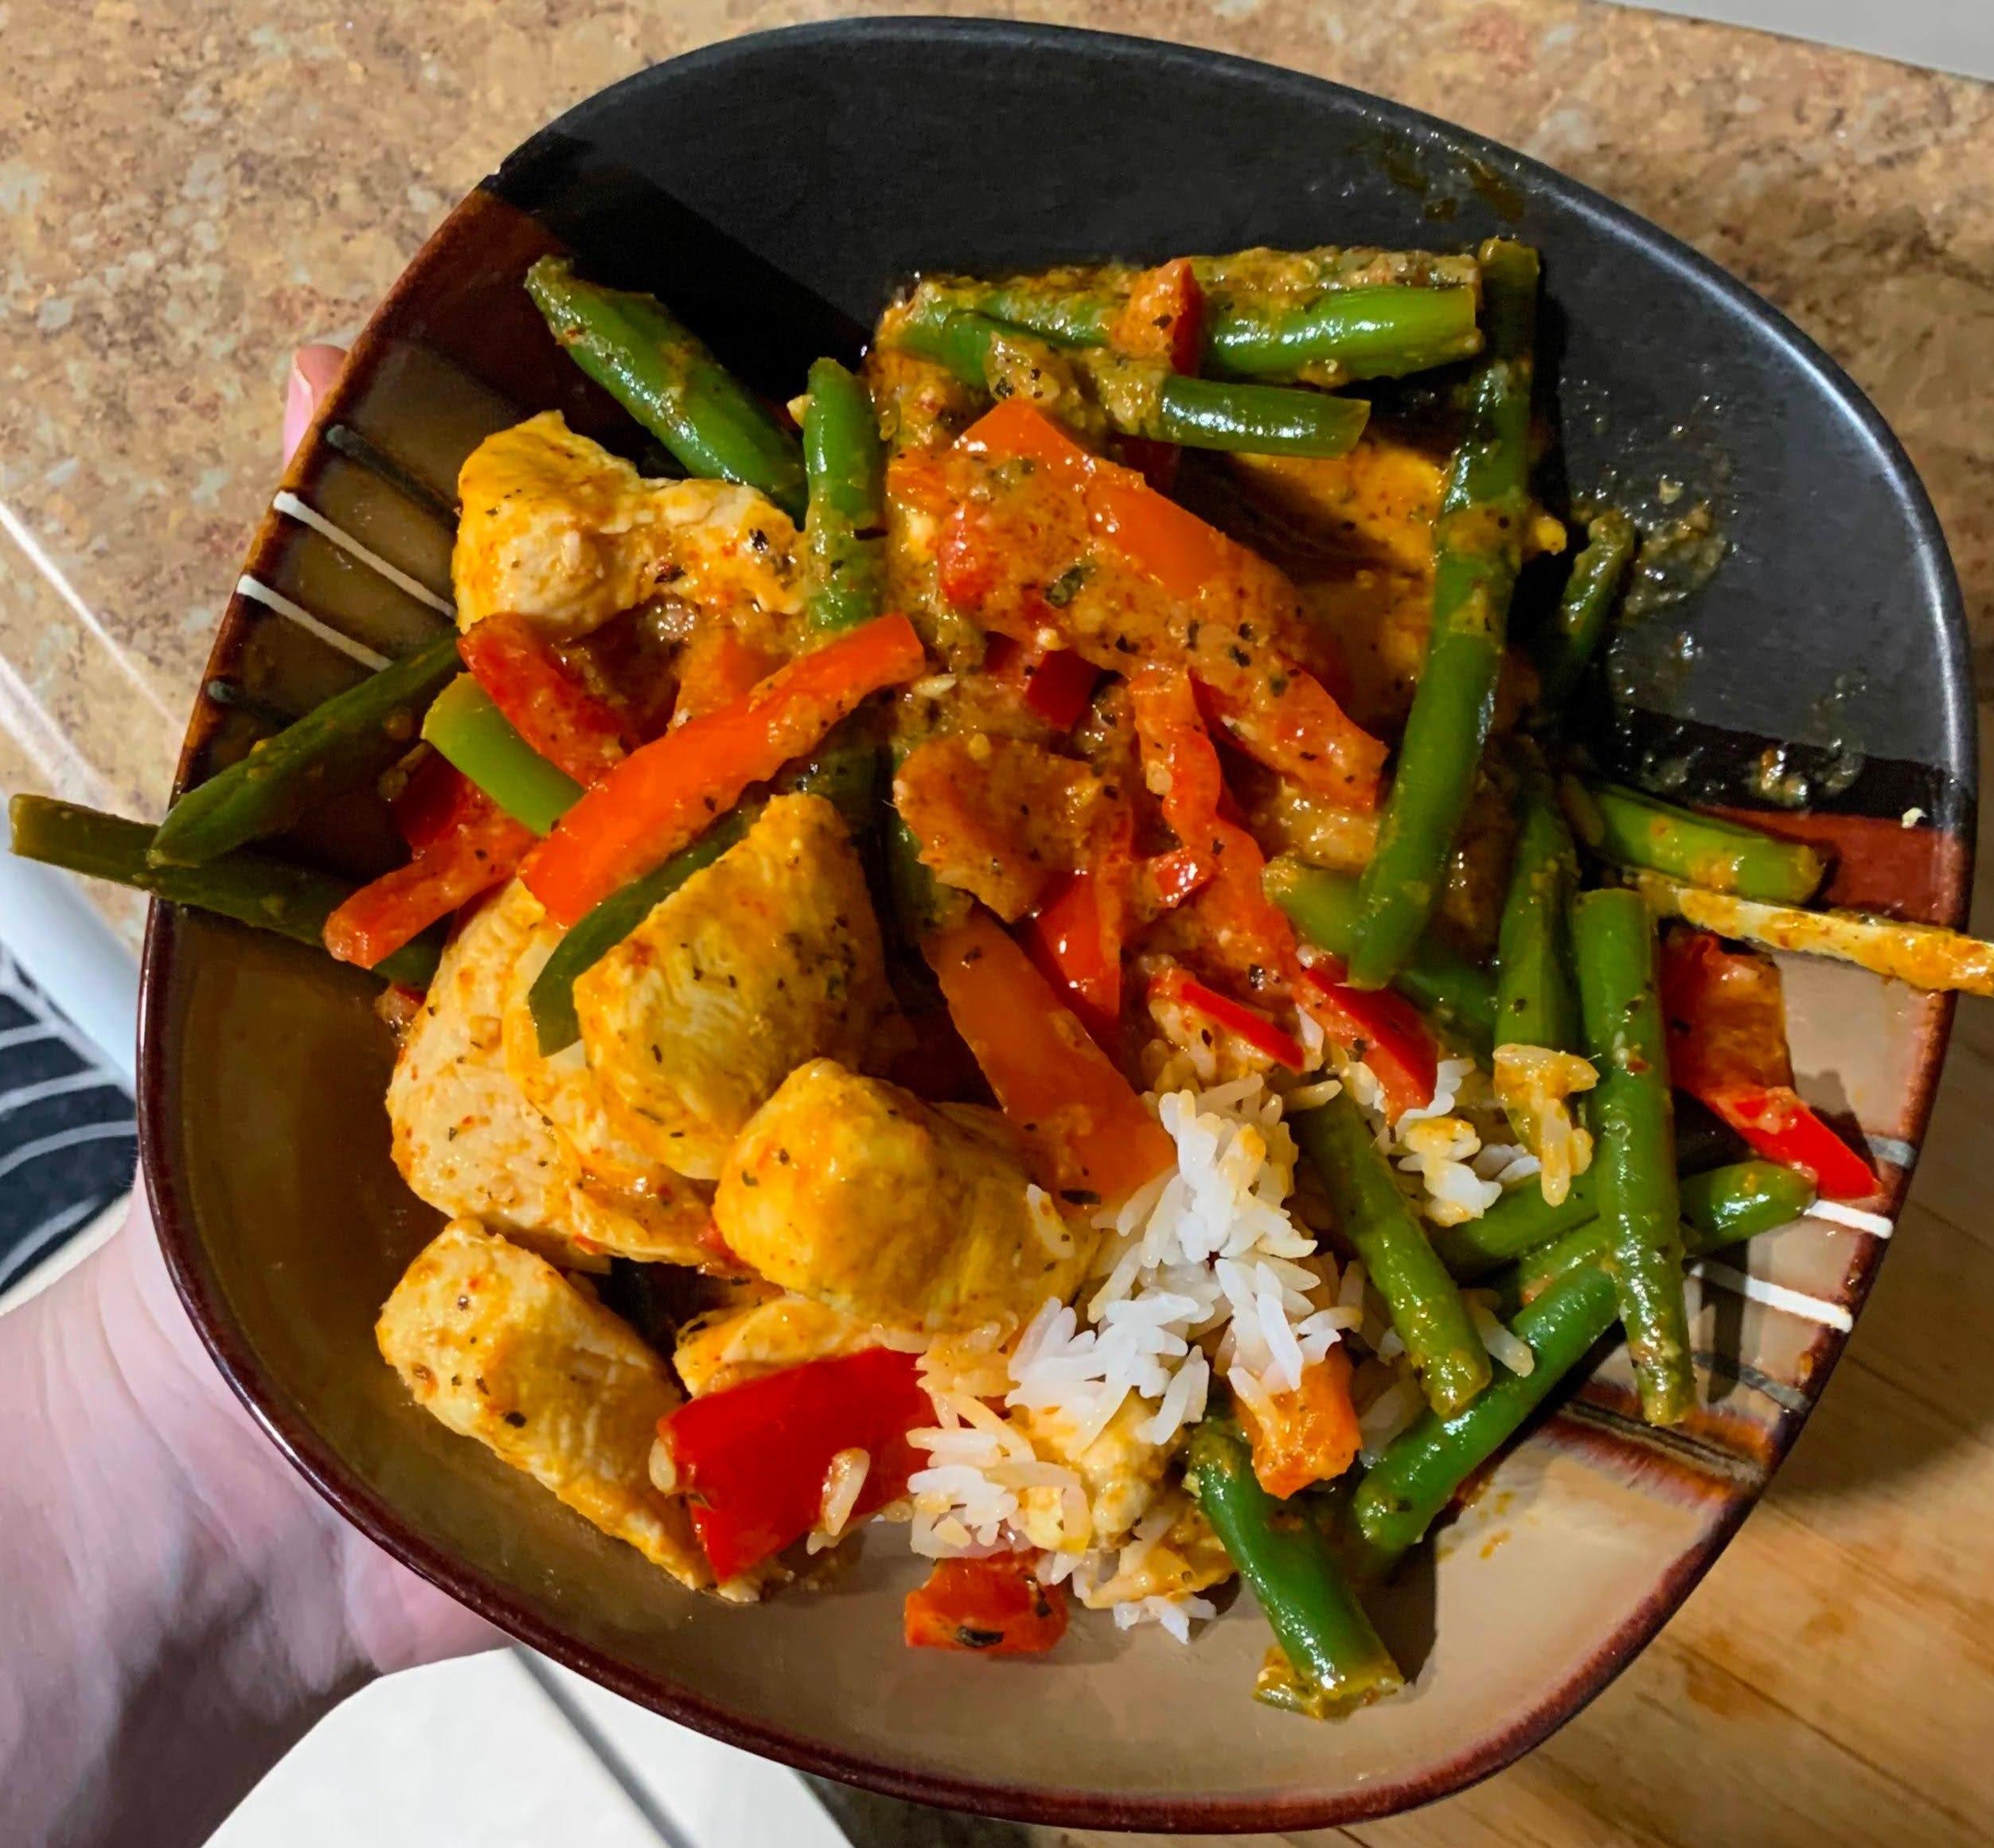
\includegraphics[scale=0.15]{Chicken Recipes/Thai Red Curry/IMG_8941-EDIT (1).jpg}

